% Options for packages loaded elsewhere
\PassOptionsToPackage{unicode}{hyperref}
\PassOptionsToPackage{hyphens}{url}
\PassOptionsToPackage{dvipsnames,svgnames,x11names}{xcolor}
%
\documentclass[
  letterpaper,
  DIV=11,
  numbers=noendperiod]{scrartcl}

\usepackage{amsmath,amssymb}
\usepackage{iftex}
\ifPDFTeX
  \usepackage[T1]{fontenc}
  \usepackage[utf8]{inputenc}
  \usepackage{textcomp} % provide euro and other symbols
\else % if luatex or xetex
  \usepackage{unicode-math}
  \defaultfontfeatures{Scale=MatchLowercase}
  \defaultfontfeatures[\rmfamily]{Ligatures=TeX,Scale=1}
\fi
\usepackage{lmodern}
\ifPDFTeX\else  
    % xetex/luatex font selection
\fi
% Use upquote if available, for straight quotes in verbatim environments
\IfFileExists{upquote.sty}{\usepackage{upquote}}{}
\IfFileExists{microtype.sty}{% use microtype if available
  \usepackage[]{microtype}
  \UseMicrotypeSet[protrusion]{basicmath} % disable protrusion for tt fonts
}{}
\makeatletter
\@ifundefined{KOMAClassName}{% if non-KOMA class
  \IfFileExists{parskip.sty}{%
    \usepackage{parskip}
  }{% else
    \setlength{\parindent}{0pt}
    \setlength{\parskip}{6pt plus 2pt minus 1pt}}
}{% if KOMA class
  \KOMAoptions{parskip=half}}
\makeatother
\usepackage{xcolor}
\setlength{\emergencystretch}{3em} % prevent overfull lines
\setcounter{secnumdepth}{-\maxdimen} % remove section numbering
% Make \paragraph and \subparagraph free-standing
\makeatletter
\ifx\paragraph\undefined\else
  \let\oldparagraph\paragraph
  \renewcommand{\paragraph}{
    \@ifstar
      \xxxParagraphStar
      \xxxParagraphNoStar
  }
  \newcommand{\xxxParagraphStar}[1]{\oldparagraph*{#1}\mbox{}}
  \newcommand{\xxxParagraphNoStar}[1]{\oldparagraph{#1}\mbox{}}
\fi
\ifx\subparagraph\undefined\else
  \let\oldsubparagraph\subparagraph
  \renewcommand{\subparagraph}{
    \@ifstar
      \xxxSubParagraphStar
      \xxxSubParagraphNoStar
  }
  \newcommand{\xxxSubParagraphStar}[1]{\oldsubparagraph*{#1}\mbox{}}
  \newcommand{\xxxSubParagraphNoStar}[1]{\oldsubparagraph{#1}\mbox{}}
\fi
\makeatother


\providecommand{\tightlist}{%
  \setlength{\itemsep}{0pt}\setlength{\parskip}{0pt}}\usepackage{longtable,booktabs,array}
\usepackage{calc} % for calculating minipage widths
% Correct order of tables after \paragraph or \subparagraph
\usepackage{etoolbox}
\makeatletter
\patchcmd\longtable{\par}{\if@noskipsec\mbox{}\fi\par}{}{}
\makeatother
% Allow footnotes in longtable head/foot
\IfFileExists{footnotehyper.sty}{\usepackage{footnotehyper}}{\usepackage{footnote}}
\makesavenoteenv{longtable}
\usepackage{graphicx}
\makeatletter
\newsavebox\pandoc@box
\newcommand*\pandocbounded[1]{% scales image to fit in text height/width
  \sbox\pandoc@box{#1}%
  \Gscale@div\@tempa{\textheight}{\dimexpr\ht\pandoc@box+\dp\pandoc@box\relax}%
  \Gscale@div\@tempb{\linewidth}{\wd\pandoc@box}%
  \ifdim\@tempb\p@<\@tempa\p@\let\@tempa\@tempb\fi% select the smaller of both
  \ifdim\@tempa\p@<\p@\scalebox{\@tempa}{\usebox\pandoc@box}%
  \else\usebox{\pandoc@box}%
  \fi%
}
% Set default figure placement to htbp
\def\fps@figure{htbp}
\makeatother

\KOMAoption{captions}{tableheading}
\makeatletter
\@ifpackageloaded{caption}{}{\usepackage{caption}}
\AtBeginDocument{%
\ifdefined\contentsname
  \renewcommand*\contentsname{Table of contents}
\else
  \newcommand\contentsname{Table of contents}
\fi
\ifdefined\listfigurename
  \renewcommand*\listfigurename{List of Figures}
\else
  \newcommand\listfigurename{List of Figures}
\fi
\ifdefined\listtablename
  \renewcommand*\listtablename{List of Tables}
\else
  \newcommand\listtablename{List of Tables}
\fi
\ifdefined\figurename
  \renewcommand*\figurename{Figure}
\else
  \newcommand\figurename{Figure}
\fi
\ifdefined\tablename
  \renewcommand*\tablename{Table}
\else
  \newcommand\tablename{Table}
\fi
}
\@ifpackageloaded{float}{}{\usepackage{float}}
\floatstyle{ruled}
\@ifundefined{c@chapter}{\newfloat{codelisting}{h}{lop}}{\newfloat{codelisting}{h}{lop}[chapter]}
\floatname{codelisting}{Listing}
\newcommand*\listoflistings{\listof{codelisting}{List of Listings}}
\makeatother
\makeatletter
\makeatother
\makeatletter
\@ifpackageloaded{caption}{}{\usepackage{caption}}
\@ifpackageloaded{subcaption}{}{\usepackage{subcaption}}
\makeatother

\usepackage{bookmark}

\IfFileExists{xurl.sty}{\usepackage{xurl}}{} % add URL line breaks if available
\urlstyle{same} % disable monospaced font for URLs
\hypersetup{
  pdftitle={TTC Subway Delay Analysis},
  pdfauthor={Omina Nematova},
  colorlinks=true,
  linkcolor={blue},
  filecolor={Maroon},
  citecolor={Blue},
  urlcolor={Blue},
  pdfcreator={LaTeX via pandoc}}


\title{TTC Subway Delay Analysis}
\author{Omina Nematova}
\date{2025-03-17}

\begin{document}
\maketitle


\paragraph{Project GitHub:
https://github.com/omina26/TTC-Subway-Delay-Analysis}\label{project-github-httpsgithub.comomina26ttc-subway-delay-analysis}

\subsubsection{Introduction}\label{introduction}

As businesses increasingly encourage employees to return to in-office
work, reliable transportation is becoming more important than ever for
commuters. Many workers rely on subway systems for their daily commutes.
Subway delays can disrupt schedules, increase travel time uncertainty,
and even influence long-term decisions about where people choose to live
or work. While some delays may be unavoidable, understanding when and
where these delays occur, as well as how external factors like weather
conditions and population density contribute to service disruptions can
help both commuters and policymakers make informed decisions.

This study investigates when and where subway delays occur within the
Toronto Transit Commission (TTC) system and analyzes the impact of
weather conditions and service population density on these delays using
a merged dataset from multiple sources. Subway delay reports (see
reference) were obtained from the City of Toronto Open Data Catalogue,
providing details on location, time, and cause of delays across the TTC
subway network. Service population estimates were derived from Toronto
Neighbourhood Profiles (see reference), also sourced from the Open Data
Catalogue, while spatial data for neighbourhoods and station locations
was incorporated using the Toronto Neighbourhoods shapefile (see
reference), TTC Subway and Streetcar Map (see reference) and
OpenStreetMap API (see reference). Additionally, hourly weather data
from 2024 was retrieved using the Open-meteo API (see reference),
allowing for an assessment of temperature, precipitation, and other
environmental factors at the time of each recorded delay.

\subsubsection{Methodology}\label{methodology}

To analyze the occurrence of subway delays and the potential impact of
weather conditions and population density, this study integrates
multiple datasets, combining transit delay reports, weather data, and
demographic information. The TTC Subway Delay Data from 2024, acquired
from the City of Toronto Open Data Catalogue, consists of 26,467 entries
with details on the date, time, day of the week, station, delay code
(cause of delay), minutes of delay, minutes of gap between trains, train
direction (bound), subway line, and vehicle ID. For this analysis, all
columns were retained except for minutes of gap between trains and
vehicle ID. To account for population density, Toronto Neighbourhood
Profiles data from 2021, also sourced from the City of Toronto Open Data
Catalogue, was incorporated. This dataset includes 158 entries with
demographic information, from which only neighbourhood ID and total
population were used to estimate the service population surrounding each
station. Additionally, Toronto Neighbourhoods shapefile data, obtained
from the City of Toronto Open Data Catalogue, contained 158 entries and
12 columns and was used for geographic mapping.

To further enrich the analysis, a custom subway station dataframe was
created by manually collecting the names of all 70 subway stations from
the TTC Subway and Streetcar Map and retrieving station longitude and
latitude coordinates using the OpenStreetMap API to allow for spatial
integration with other dataframes. Weather conditions were incorporated
using hourly weather data from 2024, retrieved from the Open-Meteo API,
which contained 8,784 entries with columns detailing the date,
temperature, relative humidity, apparent temperature, precipitation,
rain, snowfall, snow depth, cloud cover, wind speed, wind direction, and
wind gusts. All columns from this dataset were used to assess the impact
of different weather variables on subway delays.

Once collected, the datasets underwent extensive cleaning and
preprocessing to ensure consistency and usability. The TTC Subway Delay
Data, originally containing 10 columns, was filtered to remove minutes
of gap between trains and vehicle ID. Columns were renamed for clarity,
and duplicate rows or rows with null values in the bound or line columns
were removed. Subway station names were standardized, and a new hour
column was created to facilitate merging with the weather dataframe. The
day, station, code, bound, and line columns were converted to
categorical types to improve usability during analysis. Most
importantly, only observations with delays greater than zero minutes and
less than or equal to 30 minutes were retained, reducing the dataset to
9,038 rows. The population dataframe was created by filtering the
Toronto Neighbourhood Profiles data to retain only neighbourhood ID and
population estimates. In the weather dataset, null values in the snow
depth column were filled with zero, and an hour column was generated
from the date column.

Data wrangling was performed to integrate these datasets into a unified
structure. First, the Toronto Neighbourhoods shapefile was merged with
the population dataframe using neighbourhood IDs. Next, the stations
dataframe was spatially joined with the neighbourhoods shapefile to
identify neighborhoods within 0.5 km of a station, allowing service
population estimates to be merged into the stations dataframe. The delay
dataframe and weather dataframe were then merged on date and hour to
create a comprehensive dataset. Finally, service population counts for
each station were merged into this final dataset using station names as
the key identifier.

To understand patterns in subway delays, summary statistics were
computed for all numerical variables in the dataset. A histogram was
generated to visualize the distribution of delay durations, highlighting
the frequency of different delay times. The most common delay codes were
identified, and their frequency was plotted to determine the predominant
causes of disruptions. Additionally, delays were analyzed across subway
lines, train directions (bounds), and stations to assess variations in
delay occurrence by location.

Temporal analysis was conducted by examining delay frequencies and
average delay durations by hour of the day. A bar plot illustrated the
number of delays per hour, while a line plot showed fluctuations in
average delay durations throughout the day. Spatial trends were further
explored by identifying the top three stations per subway line with the
highest delay occurrences and comparing their average delay durations. A
regression analysis was performed to evaluate the relationship between
service population and delay duration, providing insights into whether
higher-density areas experience more frequent or prolonged delays.

A correlation heatmap was generated to assess relationships between
weather variables and subway delays. Finally, an ANOVA test was
conducted to determine whether delay durations significantly differed
across days of the week, stations, subway lines, and subway bounds,
offering statistical validation of observed trends.

\subsubsection{Results}\label{results}

To begin the analysis, summary statistics were computed for key
numerical variables, including subway delay durations, weather
conditions, and service population.

\begin{longtable}[]{@{}lllllllll@{}}
\caption{Table 1: Summary Statistics of Merged
Data}\label{T_7263b}\tabularnewline
\toprule\noalign{}
~ & Count & Mean & Std Dev & Min & Q1 & Median & Q3 & Max \\
\midrule\noalign{}
\endfirsthead
\toprule\noalign{}
~ & Count & Mean & Std Dev & Min & Q1 & Median & Q3 & Max \\
\midrule\noalign{}
\endhead
\bottomrule\noalign{}
\endlastfoot
Min Delay & 9028.00 & 6.56 & 4.79 & 2.00 & 4.00 & 5.00 & 7.00 & 30.00 \\
Hour & 9028.00 & 12.96 & 6.02 & 0.00 & 8.00 & 13.00 & 18.00 & 23.00 \\
Temperature & 9028.00 & 9.66 & 9.46 & -16.01 & 1.94 & 9.44 & 17.79 &
30.49 \\
Relative Humidity & 9028.00 & 73.68 & 15.41 & 21.45 & 62.80 & 75.17 &
86.09 & 100.00 \\
Apparent Temperature & 9028.00 & 7.17 & 11.79 & -21.34 & -2.51 & 6.09 &
17.18 & 33.97 \\
Precipitation & 9028.00 & 0.12 & 0.56 & 0.00 & 0.00 & 0.00 & 0.00 &
14.40 \\
Rain & 9028.00 & 0.11 & 0.55 & 0.00 & 0.00 & 0.00 & 0.00 & 14.40 \\
Snowfall & 9028.00 & 0.01 & 0.06 & 0.00 & 0.00 & 0.00 & 0.00 & 1.89 \\
Snow Depth & 9028.00 & 0.01 & 0.02 & 0.00 & 0.00 & 0.00 & 0.00 & 0.10 \\
Cloud Cover & 9028.00 & 62.90 & 41.79 & 0.00 & 15.00 & 90.00 & 100.00 &
100.00 \\
Wind Speed & 9028.00 & 13.45 & 6.73 & 0.00 & 8.43 & 12.40 & 17.69 &
39.12 \\
Wind Gusts & 9028.00 & 27.61 & 12.75 & 1.44 & 18.00 & 25.92 & 35.64 &
80.28 \\
Service Population & 9028.00 & 53200.92 & 21773.92 & 0.00 & 36845.00 &
53450.00 & 71680.00 & 105725.00 \\
\end{longtable}

In Table 1, we see that the average delay duration is around 6.56
minutes, with weather factors like temperature (avg. 9.66°C), relative
humidity (73.68\%), and wind speed (13.45 km/h) included. Precipitation
and snowfall are minimal, while service population varies widely (avg.
52,123).

Understanding the distribution of delay durations is necessary in
assessing how frequently subway delays occur and their typical length. A
histogram was generated to visualize the frequency distribution of delay
durations

\pandocbounded{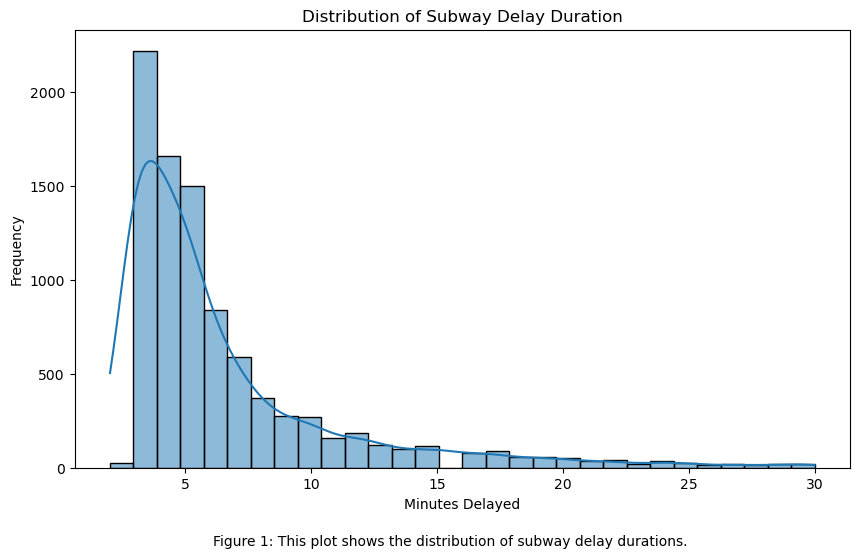
\includegraphics[keepaspectratio]{report_files/figure-pdf/cell-9-output-1.png}}

In Figure 1,it appears the distribution of subway delay durations is
left skewed with center around 5. This suggests most subway delays don't
last longer than a few minutes.

To further explore the nature of subway delays, the most common delay
codes were identified and visualized in a bar chart.

\pandocbounded{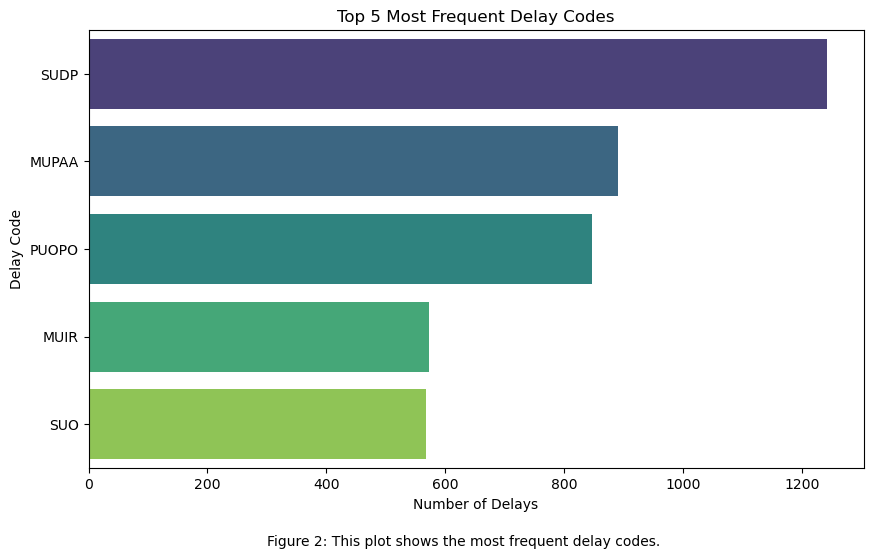
\includegraphics[keepaspectratio]{report_files/figure-pdf/cell-10-output-1.png}}

From Figure 2, we see the most frequent delay codes in our data.
According to the documentation provided in the TTC Subway Delay data
(see reference), `SUDP' is the delay code for `Disorderly Patron',
`MUPAA' is the delay code for `Passenger Assistance Alarm Activated - No
Trouble Found', `SUO' is the delay code for `Passenger Other', `PUOPO'
is the delay code for `OPTO (COMMS) Train Door Monitoring', and `MUIR'
is the delay code for `Injured or ill Customer (On Train) - Medical Aid
Refused'. All of these delay codes are possible when stations are busy
and full of commuters.

Given that different subway lines may experience varying levels of
congestion and maintenance challenges, a boxplot was used to compare the
distribution of delays across lines.

\pandocbounded{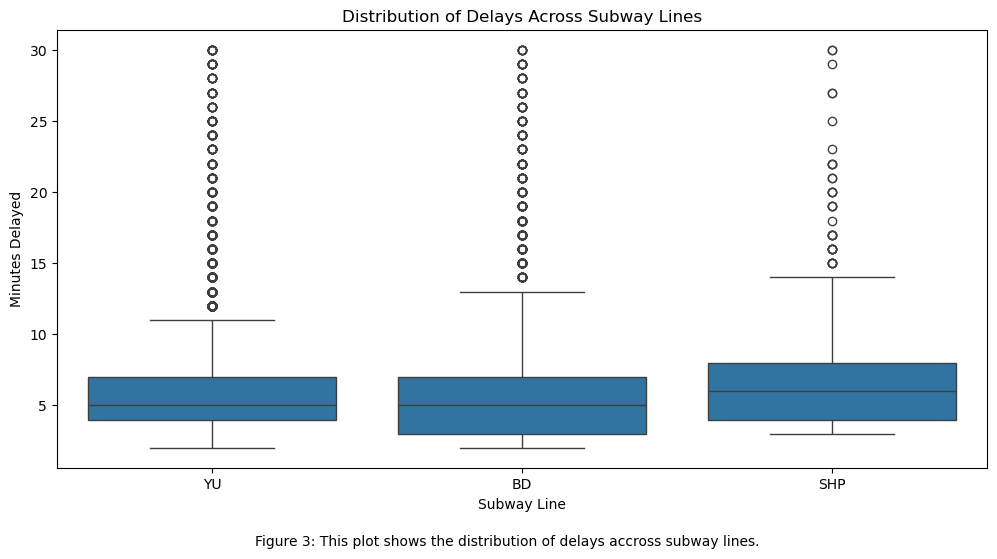
\includegraphics[keepaspectratio]{report_files/figure-pdf/cell-11-output-1.png}}

Figure 3 suggests that Sheppard (SHP) line, is more prone to prolonged
delays. Building on the subway line analysis, a bar chart was created to
highlight the three most delay-prone stations per line.

\pandocbounded{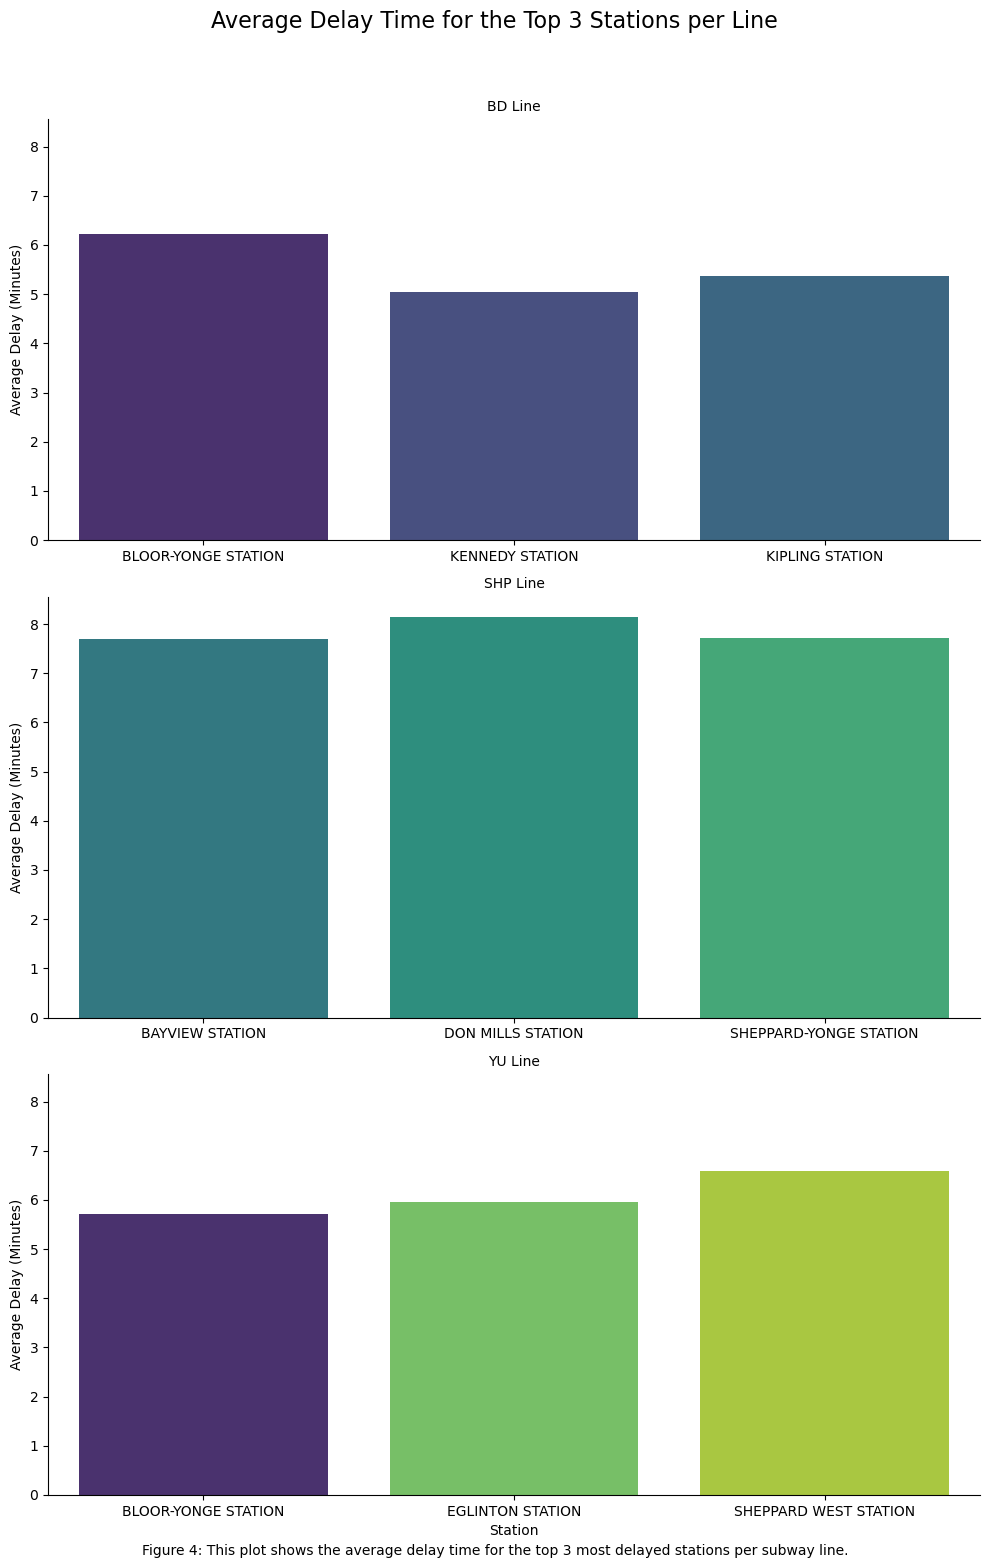
\includegraphics[keepaspectratio]{report_files/figure-pdf/cell-12-output-1.png}}

According to Figure 4, the most delayed stations on the Bloor-Danforth
(BD) line are Bloor-Yonge, Kennedy, and Kipling stations. Further, the
most delayed stations on the Sheppard (SHP) line are Bayview, Don Mills,
and Sheppard-Yonge stations. Lastly, the most delated stations on the
Yonge-University line are Bloor-Yone, Eglinton, and Sheppard West
stations. All of these stations average a delay duration of over 5
minutes.

Another dimension of analysis involves train direction, as certain
routes may be more susceptible to delays due to traffic flow or
infrastructure constraints. A boxplot was used to compare the
distribution of delays across train directions (northbound, southbound,
eastbound, westbound), identifying whether specific bounds experience
more disruptions.

\pandocbounded{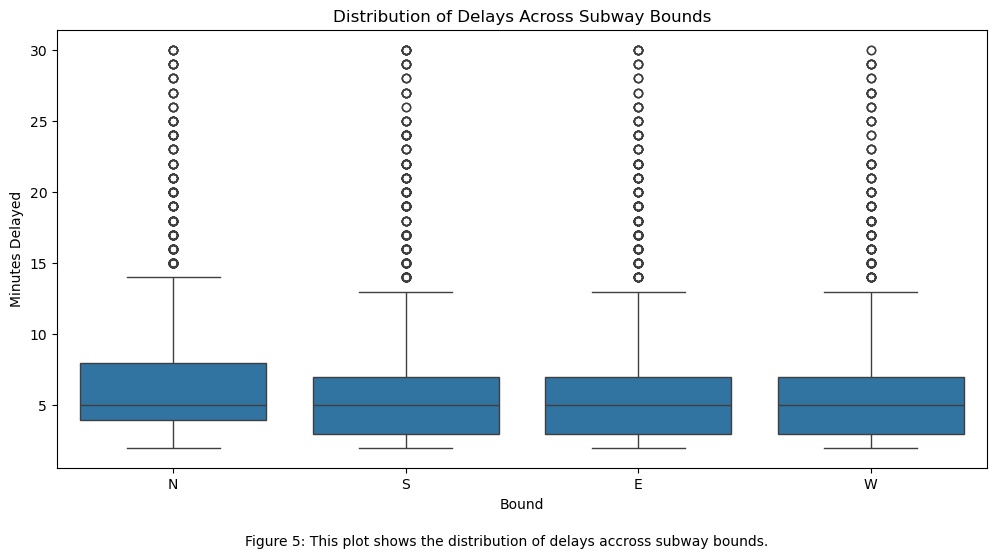
\includegraphics[keepaspectratio]{report_files/figure-pdf/cell-13-output-1.png}}

In Figure 5, it appears northbound subways are more prone to longer
disruptions with the other three having similar means and ranges.

Since subway usage fluctuates throughout the day, analyzing delays by
hour can reveal peak periods of service disruption. A bar chart was used
to visualize the number of delays occurring at each hour, helping to
pinpoint when delays are most frequent. While delay frequency is
important, understanding the average delay duration at different times
of the day provides additional insight. A line plot was also generated
to track fluctuations in average delay durations, highlighting whether
peak travel hours correspond to longer delays.

\pandocbounded{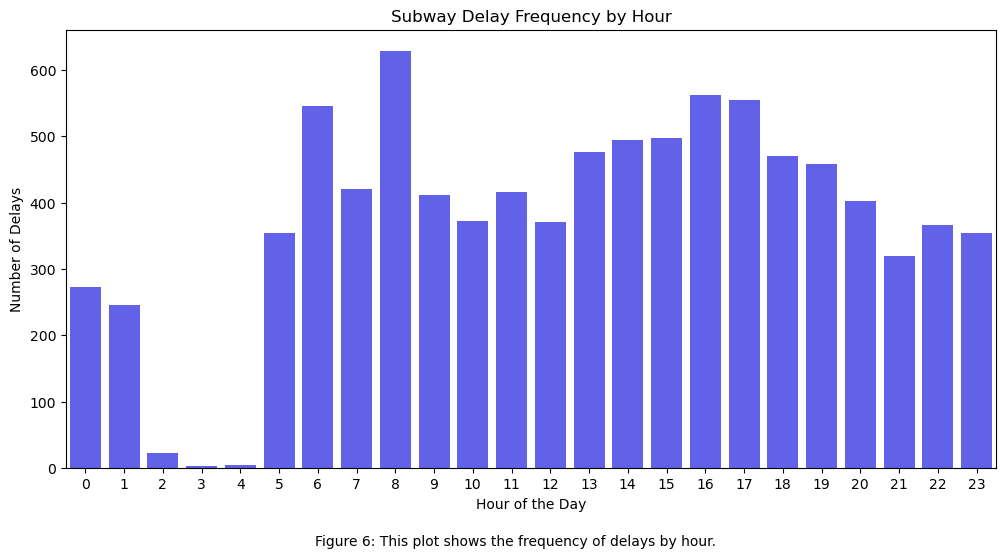
\includegraphics[keepaspectratio]{report_files/figure-pdf/cell-14-output-1.png}}

\pandocbounded{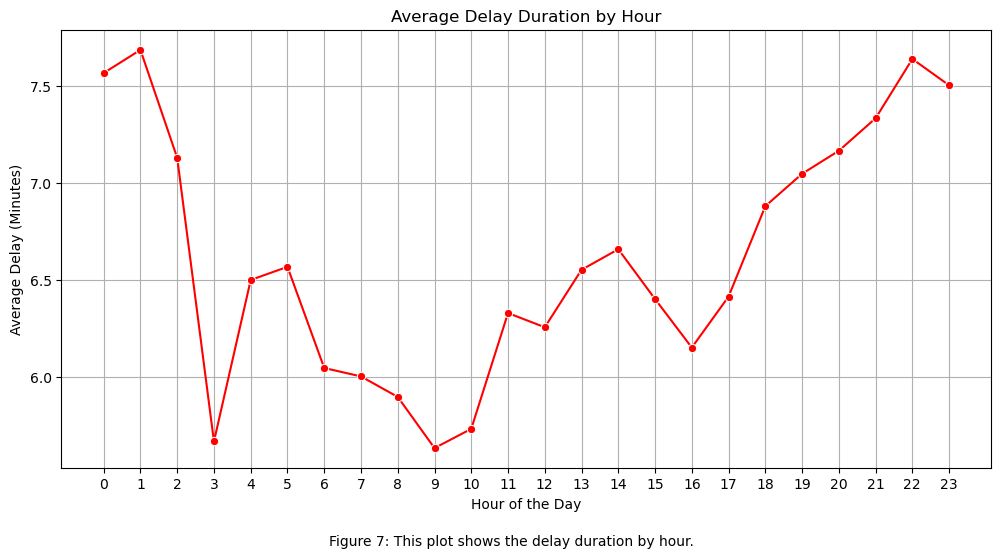
\includegraphics[keepaspectratio]{report_files/figure-pdf/cell-15-output-1.png}}

Based on Figures 6 and 7, subway delays are most frequent during morning
and afternoon rush hours. However, the average delay duration is shorter
during these periods compared to non-rush hours. This aligns with
expectations, as the TTC likely prioritizes rapid resolution of delays
during peak commuting times to minimize disruptions for the highest
volume of passengers.

Beyond daily variations, subway performance may also differ across days
of the week. A boxplot was used to visualize delay distributions for
each day, allowing for the identification of patterns that may be linked
to weekday rush hours or weekend maintenance work.

\pandocbounded{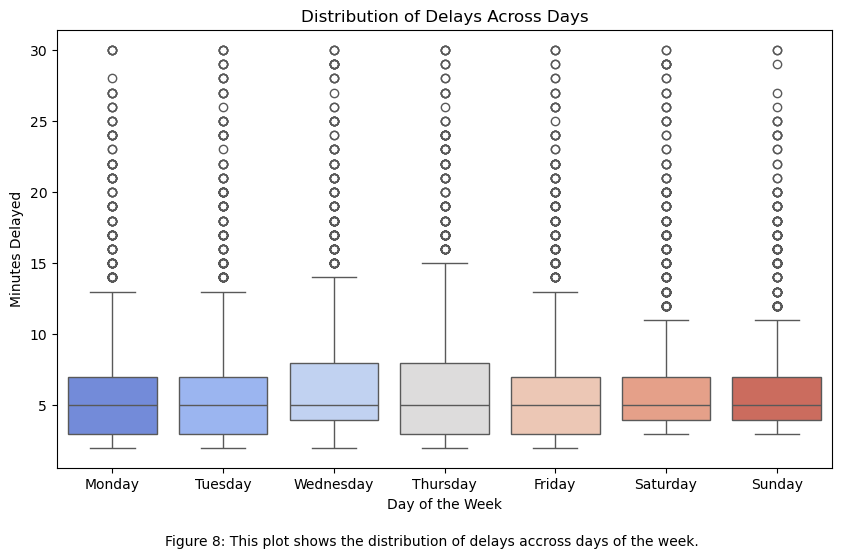
\includegraphics[keepaspectratio]{report_files/figure-pdf/cell-16-output-1.png}}

According to Figure 8, the average delay duration remains consistent
across all days of the week, but the range of delays varies. Wednesdays
and Thursdays show the widest range, while Saturdays and Sundays have
the narrowest. This may be due to higher passenger volumes on weekends,
potentially leading to longer but more consistent delays.

To further validate the observed trends, an ANOVA test was conducted to
determine whether significant differences exist in delay durations
across days, bounds, subway lines, and subway stations.

\begin{longtable}[]{@{}llllll@{}}
\caption{Table 2: ANOVA Results on the Impact of Subway Line on Delay
Time}\label{T_90897}\tabularnewline
\toprule\noalign{}
~ & Degrees of Freedom & Sum of Squares & Mean Square & F-Statistic &
p-Value \\
\midrule\noalign{}
\endfirsthead
\toprule\noalign{}
~ & Degrees of Freedom & Sum of Squares & Mean Square & F-Statistic &
p-Value \\
\midrule\noalign{}
\endhead
\bottomrule\noalign{}
\endlastfoot
Day & 6.0000 & 170.9064 & 28.4844 & 1.2722 & 0.2663 \\
Bound & 3.0000 & 364.6444 & 121.5481 & 5.4288 & 0.0010 \\
Line & 2.0000 & 269.9193 & 134.9596 & 6.0278 & 0.0024 \\
Station & 69.0000 & 5561.1966 & 80.5971 & 3.5998 & 0.0000 \\
Residual & 8947.0000 & 200319.2190 & 22.3895 & nan & nan \\
\end{longtable}

Based on the results of our ANOVA test in Table 2, bound, subway line,
and station were found to significantly affect the duration of delay as
they all three has p-values less than 0.05. On the other hand, the day
of the week was not found to significantly affect the duration of delay
as it had a p-value greater than 0.05.

To assess whether population density influences subway delays, a scatter
plot was created to examine the correlation between service population
size and delay duration. This analysis helps determine whether
higher-density areas experience longer or more frequent delays.

\pandocbounded{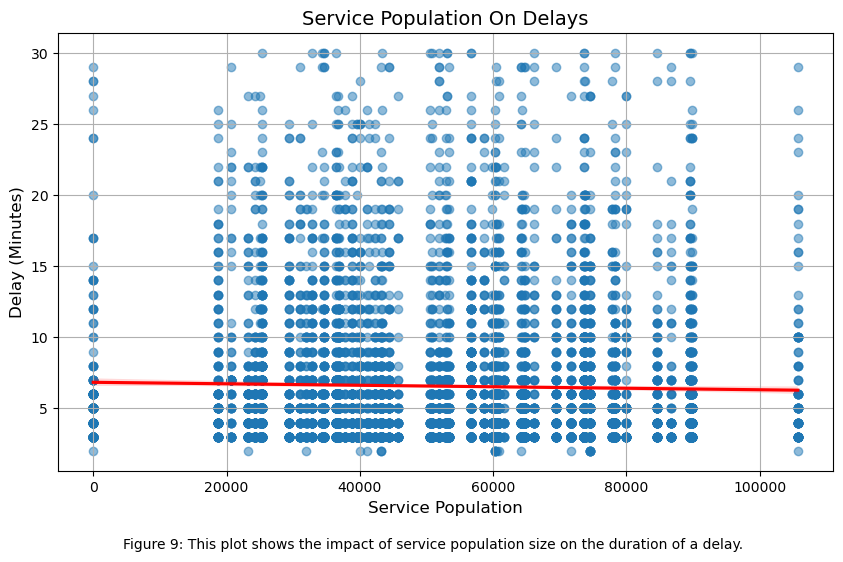
\includegraphics[keepaspectratio]{report_files/figure-pdf/cell-18-output-1.png}}

By Figure 9, the variation in delay duration appears consistent across
both high- and low-density areas. However, delays seem less frequent in
higher-density areas, as the data points are more concentrated on the
left side of the plot.

Given that transit performance is influenced by multiple factors,
weather conditions play a crucial role. To quantify this impact, a
correlation heatmap was generated to examine the relationships between
subway delays, weather conditions, and service population.

\pandocbounded{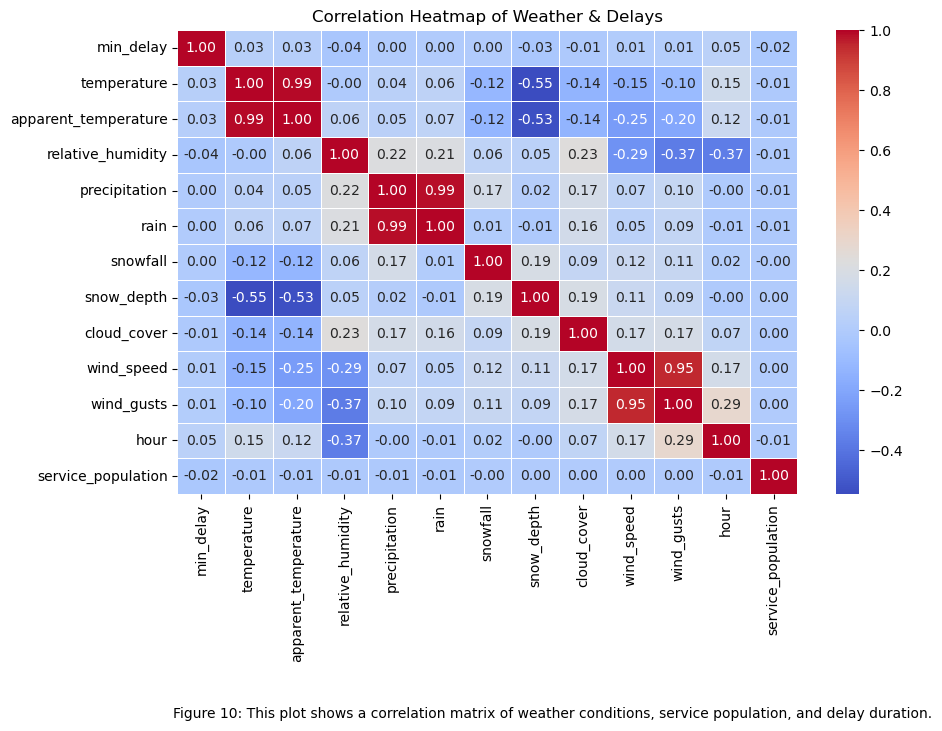
\includegraphics[keepaspectratio]{report_files/figure-pdf/cell-19-output-1.png}}

The correlation heatmap, in Figure 10, reveals that weather conditions
have minimal correlation with subway delay duration. Most weather
variables show near-zero correlations with delay duration, while
precipitation, rain, and snowfall show zero correlation, suggesting that
weather may not be a strong predictor of delay length. Additionally,
service population also has little correlation with delay duration,
indicating that population density near stations does not significantly
impact the length of delays. However, expected strong correlations are
observed between related weather variables, such as temperature and
apparent temperature, as well as precipitation and rain.

\subsubsection{Summary}\label{summary}

This study analyzed subway delays within the Toronto Transit Commission
(TTC) system, examining their occurrence and potential influences from
weather conditions and population density. Using a merged dataset of
transit delay reports, hourly weather data, and demographic information,
key patterns in delay frequency and duration were explored. The findings
indicate that delays are most frequent during morning and afternoon rush
hours, but their durations tend to be shorter compared to non-peak
times. Passenger-related incidents were the most common causes of
delays, and the Sheppard (SHP) Line experienced the longest delays.
Directional patterns also emerged, with northbound trains facing more
frequent disruptions. However, weather conditions and service population
density showed little correlation with delay duration, suggesting other
operational factors play a larger role.

To build on these findings, the next phase will involve developing
machine learning models to predict subway delays. Both classification
and regression models will be explored, including decision trees,
logistic regression, gradient boosting models. Classification models
will be used to determine whether a delay will occur based on historical
conditions, while regression models will estimate the expected duration
of a delay. By implementing predictive modeling, this study aims to
create a data-driven framework for anticipating delays, helping transit
planners optimize scheduling and commuters make informed travel
decisions.

\subsubsection{References}\label{references}

\begin{itemize}
\tightlist
\item
  Open-meteo documentation:
  \url{https://open-meteo.com/en/docs/historical-weather-api}
\item
  OpenStreetMap API documentation:
  \url{https://wiki.openstreetmap.org/wiki/API_v0.6}
\item
  Toronto Neighbourhood Profiles:
  \url{https://open.toronto.ca/dataset/neighbourhood-profiles/}
\item
  Toronto Neighbourhoods:
  \url{https://open.toronto.ca/dataset/neighbourhoods/}
\item
  TTC Subway and Streetcar Map:
  \url{https://cdn.ttc.ca/-/media/Project/TTC/DevProto/Images/Home/Routes-and-Schedules/Landing-page-pdfs/TTC_SubwayStreetcarMap_2021-11.pdf?rev=909317034177450b8b09ba5b247e24bf}
\item
  TTC Subway Delay Data:
  \url{https://open.toronto.ca/dataset/ttc-subway-delay-data/}
\end{itemize}




\end{document}
